\documentclass[a4paper, 12pt]{article}
\usepackage[brazilian]{babel} %pacote babel para tweaks em relaçao à linguagem
\usepackage{amsmath}
\usepackage[utf8]{inputenc} %acentos e carácteres específicos
\usepackage[scaled]{helvet}
\renewcommand\familydefault{\sfdefault}
\usepackage[T1]{fontenc}
\usepackage{csquotes} %csquotes auxilia babel
\usepackage[
bottom=2cm,
top=3cm,
left=3cm,
right=2cm,
]{geometry}  %geometry para definição das margens
\usepackage{indentfirst} %primeiro parágrafo "indentado"
\usepackage{tkz-graph} %tkz-graph para criação de grafos
\usepackage{multicol}%para várias colunas
\usepackage{graphicx}

\begin{document}
\title{\textbf{Teoria dos Grafos}\\ \small{Grafos, segunda parte: Grafos Eulerianos e o Algoritmo de Dijkstra}}
\author{Leon Ferreira Bellini\\
	\small{\textbf{RA\@ 22218002--8}}\\
	e\\
   Guilherme Ormond Sampaio\\
   \small{\textbf{RA\@ 22218007--7}}
}
\date{}
\maketitle
\section{Introdução}
Desde a elaboração do primeiro relatório, conteúdo relevante foi acrescentado ao nosso repertório, como caminhos, trilhas e passeios por um grafo, árvores, grafos conexos e grafos isomorfos, contudo, os objetos em foco são os grafos Eulerianos e o algoritmo de Dijsktra, o qual propõe uma resolução para o problema do caminho de peso mínimo.

\section{Conceitos Eulerianos}
Muitos dos teoremas inicialmente denotados por \textbf{Leonard Paul Euler} se utilizam dos conceitos relacionados a passeios e suas derivações, como o \textbf{Tour de Euler}, este sendo diretamente ligado ao \textbf{grafo de Euler} e por fim,  \textbf{percurso pré-Euleriano}. Serão explicados a seguir:

\subsection{O Tour ou cadeia de Euler}
Passeios de uma forma geral, podem ser abertos ou fechados, tours são caminhos fechados os quais incluem toda aresta do grafo em questão, já o \textbf{Tour de Euler} requere que a aresta apareça apenas uma vez no passeio fechado.

\subsection{Grafo Euleriano}

Um grafo \textbf{G} = (V, E) é euleriano se apresenta um ciclo (caminho fechado) que contenha todas as arestas deste \textbf{G}. A presença de um tour de euler também configura um grafo como euleriano. Outro importante fato a se notar é o que grafos eulerianos não possuem graus ímpares e a presença de uma trilha de euler não o torna um grau euleriano se este possuir grau (s) ímpar (es). 

\begin{figure}[!hbt]
        \begin{center}
            \begin{tikzpicture}[scale=1]
                \tikzset{LabelStyle/.style= {fill = white}}
                \Vertex[x=-1, y=0]{V1}
                \Vertex[x=1, y=1]{V2}
                \Vertex[x=3, y=0]{V3}
                \Vertex[x=5, y=1]{V4}
		\Vertex[x=5, y=-1]{V5}
                \Vertex[x=0, y=-2]{V6}
                \Vertex[x=2, y=-2]{V7}
                \Edge(V1)(V2)
		\Edge(V1)(V7)
		\Edge(V1)(V3)
                \Edge(V1)(V6)
                \Edge(V2)(V3)
                \Edge(V2)(V7)
                \Edge(V2)(V6)
                \Edge(V3)(V4)
                \Edge(V3)(V6)
                \Edge(V3)(V7)
                \Edge(V3)(V5)
                \Edge(V5)(V4)
		\Edge(V6)(V7)

            \end{tikzpicture}
            \caption{Exemplo de grafo Euleriano, note que todos os vértices têm índice par}

        \end{center}
    \end{figure}
    


\newpage\subsection{O percurso pré-euleriano}
Desta vez relacionado à quantidade de arestas, é o percurso que passa
em todas arestas do grafo \textbf{G}.

\begin{center}

	\begin{figure}[!hbt]
		\centering
		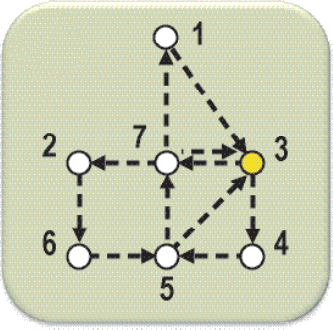
\includegraphics[width=5cm, height= 5cm]{preeuler.png}

	\caption{Grafo de sequência 3-7-1-3-4-5-3-7-2-6-5-7-3 se configura como pré euleriano -- Grafos: Conceitos, algoritmos e aplicações (2014) }
	\end{figure}

\end{center}


\section{O algoritmo de Dijkstra}
Um grafo \textbf{G} = (V, E) é ponderado quando pesos são dados a cada aresta. Também chamados de custos, o intuito é definir a partir de valores numéricos a disponibilidade, tempo, dificuldade, etc.\ de viajar de uma aresta para outra. Será necessário, primeiro, introduzir o conceito de \textbf{Grafos Ponderados}.
\subsection{Grafos ponderados}

São grafos que possuem pesos associados aos seus vértices ou arestas, tais pesos podem demonstrar certo valor relevante para a realização de um passeio ou percurso.

\begin{figure}[!hbt]
        \begin{center}
            \begin{tikzpicture}[scale=1]
                \tikzset{LabelStyle/.style= {fill = white}}
                \Vertex[x=-1, y=0]{V1}
                \Vertex[x=1, y=0]{V2}
                \Vertex[x=-3, y=-2]{V3}
                \Vertex[x=0, y=-2]{V4}
		\Vertex[x=3, y=-2]{V5}
                \Vertex[x=2, y=-5]{V6}
		\Edge[label= 3](V1)(V2)
		\Edge[label= 5](V1)(V3)
		\Edge[label= 7](V1)(V4)
		\Edge[label= 3](V2)(V4)
		\Edge[label= 1](V2)(V5)
		\Edge[label= 1](V3)(V4)
		\Edge[label= 2](V3)(V6)
		\Edge[label= 6](V4)(V6)
		\Edge[label= 1](V4)(V5)
		\Edge[label= 3](V5)(V6)

            \end{tikzpicture}
	    \caption{Exemplo de ponderação de grafo}

        \end{center}
    \end{figure}

\newpage
\subsection{O algoritmo}

NA figura 3, vamos considerar a necessidade de se transportar do vértice V1 para o vértice V4. Partindo somente da análise da quantidade de arestas o caminho V1V4 seria, de fato, o mais rápido; porém, se levarmos em consideração os pesos, não seria o mais otimizado, visto que esse mesmo vértice tem peso 7. Sendo assim, o caminho com menor peso seria V1V2V5V4, com peso 5. 

Esse problema é conhecido como problema do custo mínimo, ou problema do peso mínimo, e o Algoritmo de Dijkstra trata exatamente da resolução desse problema.

Teorizado pelo holandês Edsger Dijkstra, teria o objetivo de resolver problemas relacionados ao caminho mais curto num grafo simples direcionado ou não. Deve ser aplicado em grafos que contenham arestas de peso não negativo, porém, é possível adicionar um valor único que deixe todas arestas positivas.

\newpage
\section{Conclusão}

Ambos os temas abordados neste relatório são de extrema importância para a estruturação de dados e técnicas relacionadas, tendo o algoritmo de Dijkstra como destaque. Sua utilidade varia desde a aplicação em algoritmos ainda mais extensos para redes sociais até engenharia de tráfego e algoritmos que tenham a função de determinar o caminho mais curto de uma rede de estradas. Apesar disso, o procedimento ainda apresenta uma ineficiência quanto a grafos não direcionados ou grafos que possuam \textit{dead ends}.

\section{Referências bibliográficas}

\medskip GOLDBARG, Marco e Elizabeth. \textbf{Grafos: Conceitos, algoritmos e aplicações.}1.ed.- São Paulo: Elsevier,2012.

\medskip Dijkstra Algorithm. Direção de Computerphile. Inglaterra: Setor de Ciência da computação da Universidade de Nottingham, 2017. Disponível em: \\<https://www.youtube.com/watch?v=GazC3A4OQTE>. Acesso em 18 mai. 2019.


\medskip Grafos Eulerianos. Universidade Federal de Santa Catarina. Disponível em:\\ <http://www.inf.ufsc.br/grafos/temas/euleriano/euleriano.htm>. Acesso em 18 mai. 2019. 

\end{document}
